\section{Love \& Fear - Tantra in daily life}

\begin{center}
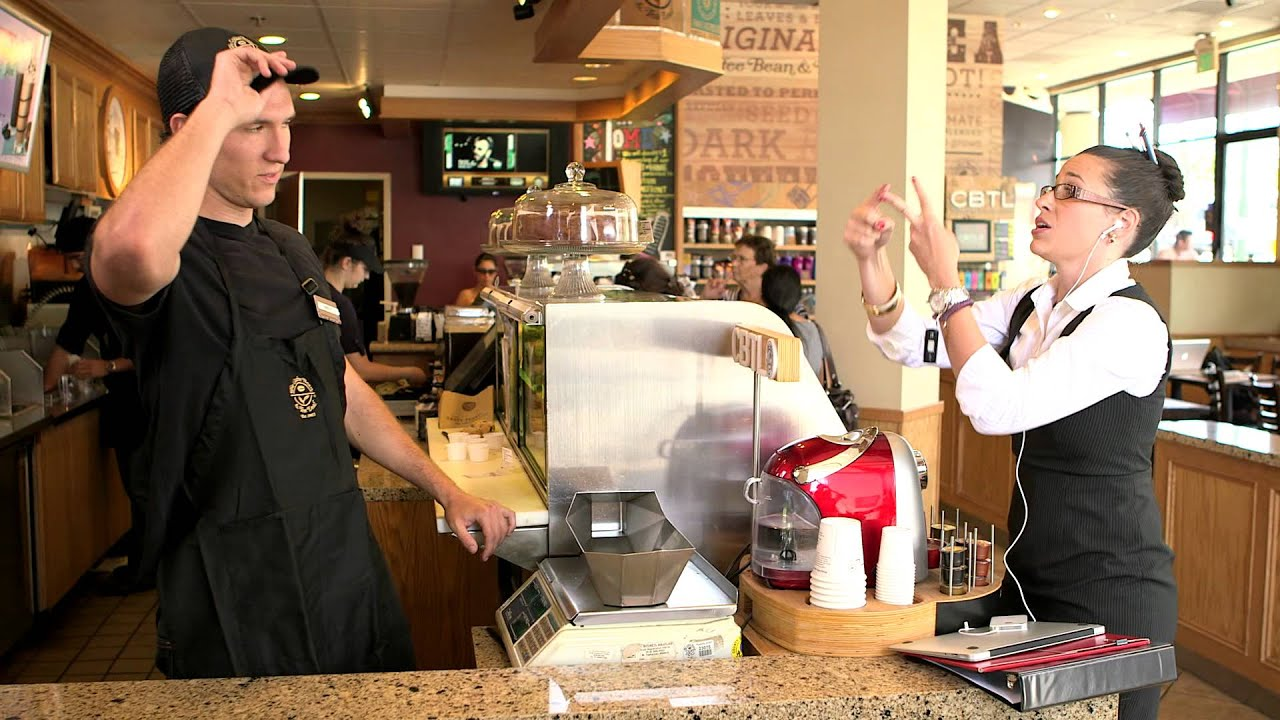
\includegraphics[width=7cm]{images/21_fear.png}
\end{center}

I am sitting in something like a coffee house in Ottawa (it's cumbersome to find sophisticated coffee houses here in the capital of Canada, but Viennese people won't let go of their high expectations so easily) and I am reading a book. About enlightenment. Instant-enlightenment, to be precise, because who has got time these days?

The book tries to justify its title and dares to ask me already on page nine to simply love everyone. I look around and try my best. A young couple with a baby. That's easy! A group of students, everyone with their laptops in front of them, discussing something passionately. Love? Yes, that should work. A couple, whose silhouettes are drawn in front of the window. He is slim and has long hair, she is firmly built, the seam of her jeans gets tense as she bends over the backgammon board. To love... hm... Why am I hesitating? What makes her less worth loving? Less for sure than the white haired grandpa with glasses just next to me, who looks like he could tell me a good night story anytime. To love babies is foolproof. Everyone can do that. They don't talk back, and when they do, I still have a lot of room for interpretation. Babies also won't challenge my worldview, at least as long as I don't engage in a serious philosophical discussion with them.

When I entered this coffee shop, I naturally sat down on a small table and waited for a moment. That's how I am used to doing it, and that's the way it is supposed to be. A coffee shop is where you wait for the waiter. After a while of waiting, I realized that the rules are different here and wondered whether I should ask the young parents about those rules. It would have been very simple: "Tell me, is someone coming to the tables, or do I have to take care of my coffee myself?"

I didn't ask. No, not because I suddenly showed a supposedly typical masculine behavior. I just didn't want to embarrass myself. (Well... When I think about it, isn't that exactly the reason for this archetypical resistance to ask strangers for directions?)

I somehow take it for granted, of course (Of course! Ha! Blessed be my upbringing!), that I simply have to know everything. Well, at least if I want to be lovable. No, just don't be perceived as lovable. Literally, to be worth of love (German: "liebenswert" or "des Liebens wert sein").

I then walked to the counter and studied first what I could order which would neither bring up my heart rate (a big black coffee) nor be too sweet (a hot chocolate) and not be too difficult to pronounce (a Macchiato), either. After some time, I decided to go for a latte. This choice corresponded with my preference for milk with a shot of coffee. I hoped that it would be understood linguistically, even if no one knows for sure how this word really is pronounced in English.

And indeed the guy behind the counter asked back. Not once. Not twice. At the third time, I observed myself how I involuntarily gestured and pointed at the big board with firm and slow gestures, just the way I would use them when interacting with a drunk person.

\textit{What's the matter? Is he deaf, do I speak Chinese, or am I too stupid to order a coffee?}

Only after the third time, and after the dark eyed guy on the other side started to use the drunken strategy himself, I suddenly realized that he had already asked the second time about my desired size of my latte.

I was just not able to love him. But why? Love seems to be so much easier when I'm not afraid. This fear doesn't have to be proper panic. A simple discomfort or the feeling of not being enough is totally sufficient.

I somehow felt a bit stupid with this guy -I didn't even manage to order a coffee for the first time- and that brought me into a defense mode. I first had to overcome my inner blushing and the beating-myself-up, so basically I had to pet myself and get upright, before I had the capacity to encounter him on the same level and simply love him.

And that's how I also felt towards the others, except maybe the babies. The students? Huh, all looked so intellectual... and my own times at the university had been 25 years in the past already. Who knows whether I could have kept up with their conversation. Especially in English. Speaking several languages on a sophisticated level that allows having a debate and owning an academic title unfortunately didn't help at all at this moment.

So back then there was no way to manage that thing about loving others. I first have to take care of myself and feel equal with them. But when I think properly about it, this won't work after all: to simply love people, because there is always someone who is more experienced, more brilliant, creative or superior in some area than me. What if I simply have to accept that? Can I then let go of this annoying fear and the exhausting thought of \textit{I-am-not-worth-loving}? Somehow it would be nice to just sit here, unpretentiously and in a relaxed way, enjoying my successfully acquired latte and to look at those people... and without them even taking notice of it, to simply love them. Being totally relaxed. Because, who knows... Maybe someone loves me back just at this very moment.

Exactly like this: Totally -- relaxed.
